
\chapter{Systementwurf}

In diesem Kapitel wird ein Entwurf für die Implementation des Systems aufgezeigt.
Die Struktur des Systems wird durch einen Architekturentwurf visualisiert und die zu verwendeten Technologien erläutert.

\section{Kein ASN.1 Compiler für Rust}
\label{draft:no_asn_compiler}

Eine frühe Recherche hat ergeben, dass kein ASN.1 Compiler für Rust verfügbar ist.
Mit \textit{yasna}, \textit{raisin} und \textit{rust-asn1} wird teilweise ASN.1 Funktionalität in Rust zur Verfügung gestellt, aber keine dieser Crates unterstützt die benötigte UPER Codierung.
Auch kann keine der genannten Crates die in ASN.1 Notation definierten Nachrichten in native Rust Datenstrukturen übersetzten.
Die von der ITU genannten Compiler\footnote{\url{https://www.itu.int/en/ITU-T/asn1/Pages/Tools.aspx}} unterstützen Rust auch nicht.
Dieser Umstand erzwingt die Nutzung der C-Datenstrukturen, wie die Referenzimplementierung, mittels \gls{ffi} (siehe \autoref{rust:ffi}).
Zur besseren Kapselung ist die Einbindung der ASN.1 Nachrichten deswegen in mehreren Schritten in zwei Crates ausgelagert.

\section{Framework Tokio}
\label{design:tokio}

Das Framework Tokio wird als Grundlage für die Umsetzung der Architektur genutzt.
Tokio\footnote{\url{https://crates.io/crates/tokio}} bietet eine \enquote{Laufzeit zum Schreiben von zuverlässigen, asynchrone und schlanke Anwendungen in Rust} \cite{rust:crate:tokio}.

Tokio nutzt die Crates \textit{mio} und \textit{Future}, um eine ereignisorientierte, asynchrone und daher nicht blockierende Ein-/Ausgabeplattform zu bieten.
Bearbeitungsschritte sind in \enquote{Futures} (dt. Zukunft, hier in etwa: \enquote{ein zukünftiger Wert}) aneinandergereiht und verpackt.

Neben den genannten technischen Funktionen ist hervorzuheben, dass das Framework von vielen Entwicklern aus dem Rust-Entwicklerteam mindestens mitentwickelt wird\footnote{u.a. Alex Crichton, Carl Lerche, Aaron Turon: \url{https://github.com/tokio-rs/tokio/graphs/contributors}}.
Aufgrund dessen ist ein hoher Grad an Qualität und Aktualität des Frameworks zu erwarten.
%Daher ist ein höherer Grad an Vertrauen in Qualität, Funktionstüchtigkeit und Aktualität gegeben.

%\section{Rust Version 1.26}
%\todo{nötig? impl ..., }


\section{Architektur}
		
In \autoref{draft:architecture} ist der Entwurf der Architektur visualisiert.
Blau markierte Klassen haben als Aufgabengebiet die Kommunikation, grün markierte Klassen bilden die Geschäftslogik ab und rot markierte Klassen sind Spezialisierungen für ASN.1.
Die folgenden ASN.1 Nachrichten sind aufgrund der Textlänge im Diagramm abgekürzt:
\begin{itemize}
	\item \textbf{asn::CR}: \textit{ClientRegistration}-Nachricht (siehe \autoref{msg:client_registration}),
	\item \textbf{asn::IM}: \textit{InitMessage}-Nachricht (siehe \autoref{msg:init_message}),
	\item \textbf{asn::US}: \textit{UpdateSubscription}-Nachricht (siehe \autoref{msg:update_subscription}),
	\item \textbf{asn::EF}: \textit{EnvironmentFrame}-Nachricht (siehe \autoref{msg:environment_frame}),
	\item \textbf{asn::SIF}: \textit{SensorIdleFrame}-Nachricht (siehe \autoref{msg:sensor_idle_frame}) und
	\item \textbf{asn::SF}: \textit{SensorFrame}-Nachricht (siehe \autoref{msg:sensor_frame}).
\end{itemize}


\begin{figure}[H]
	\centering
	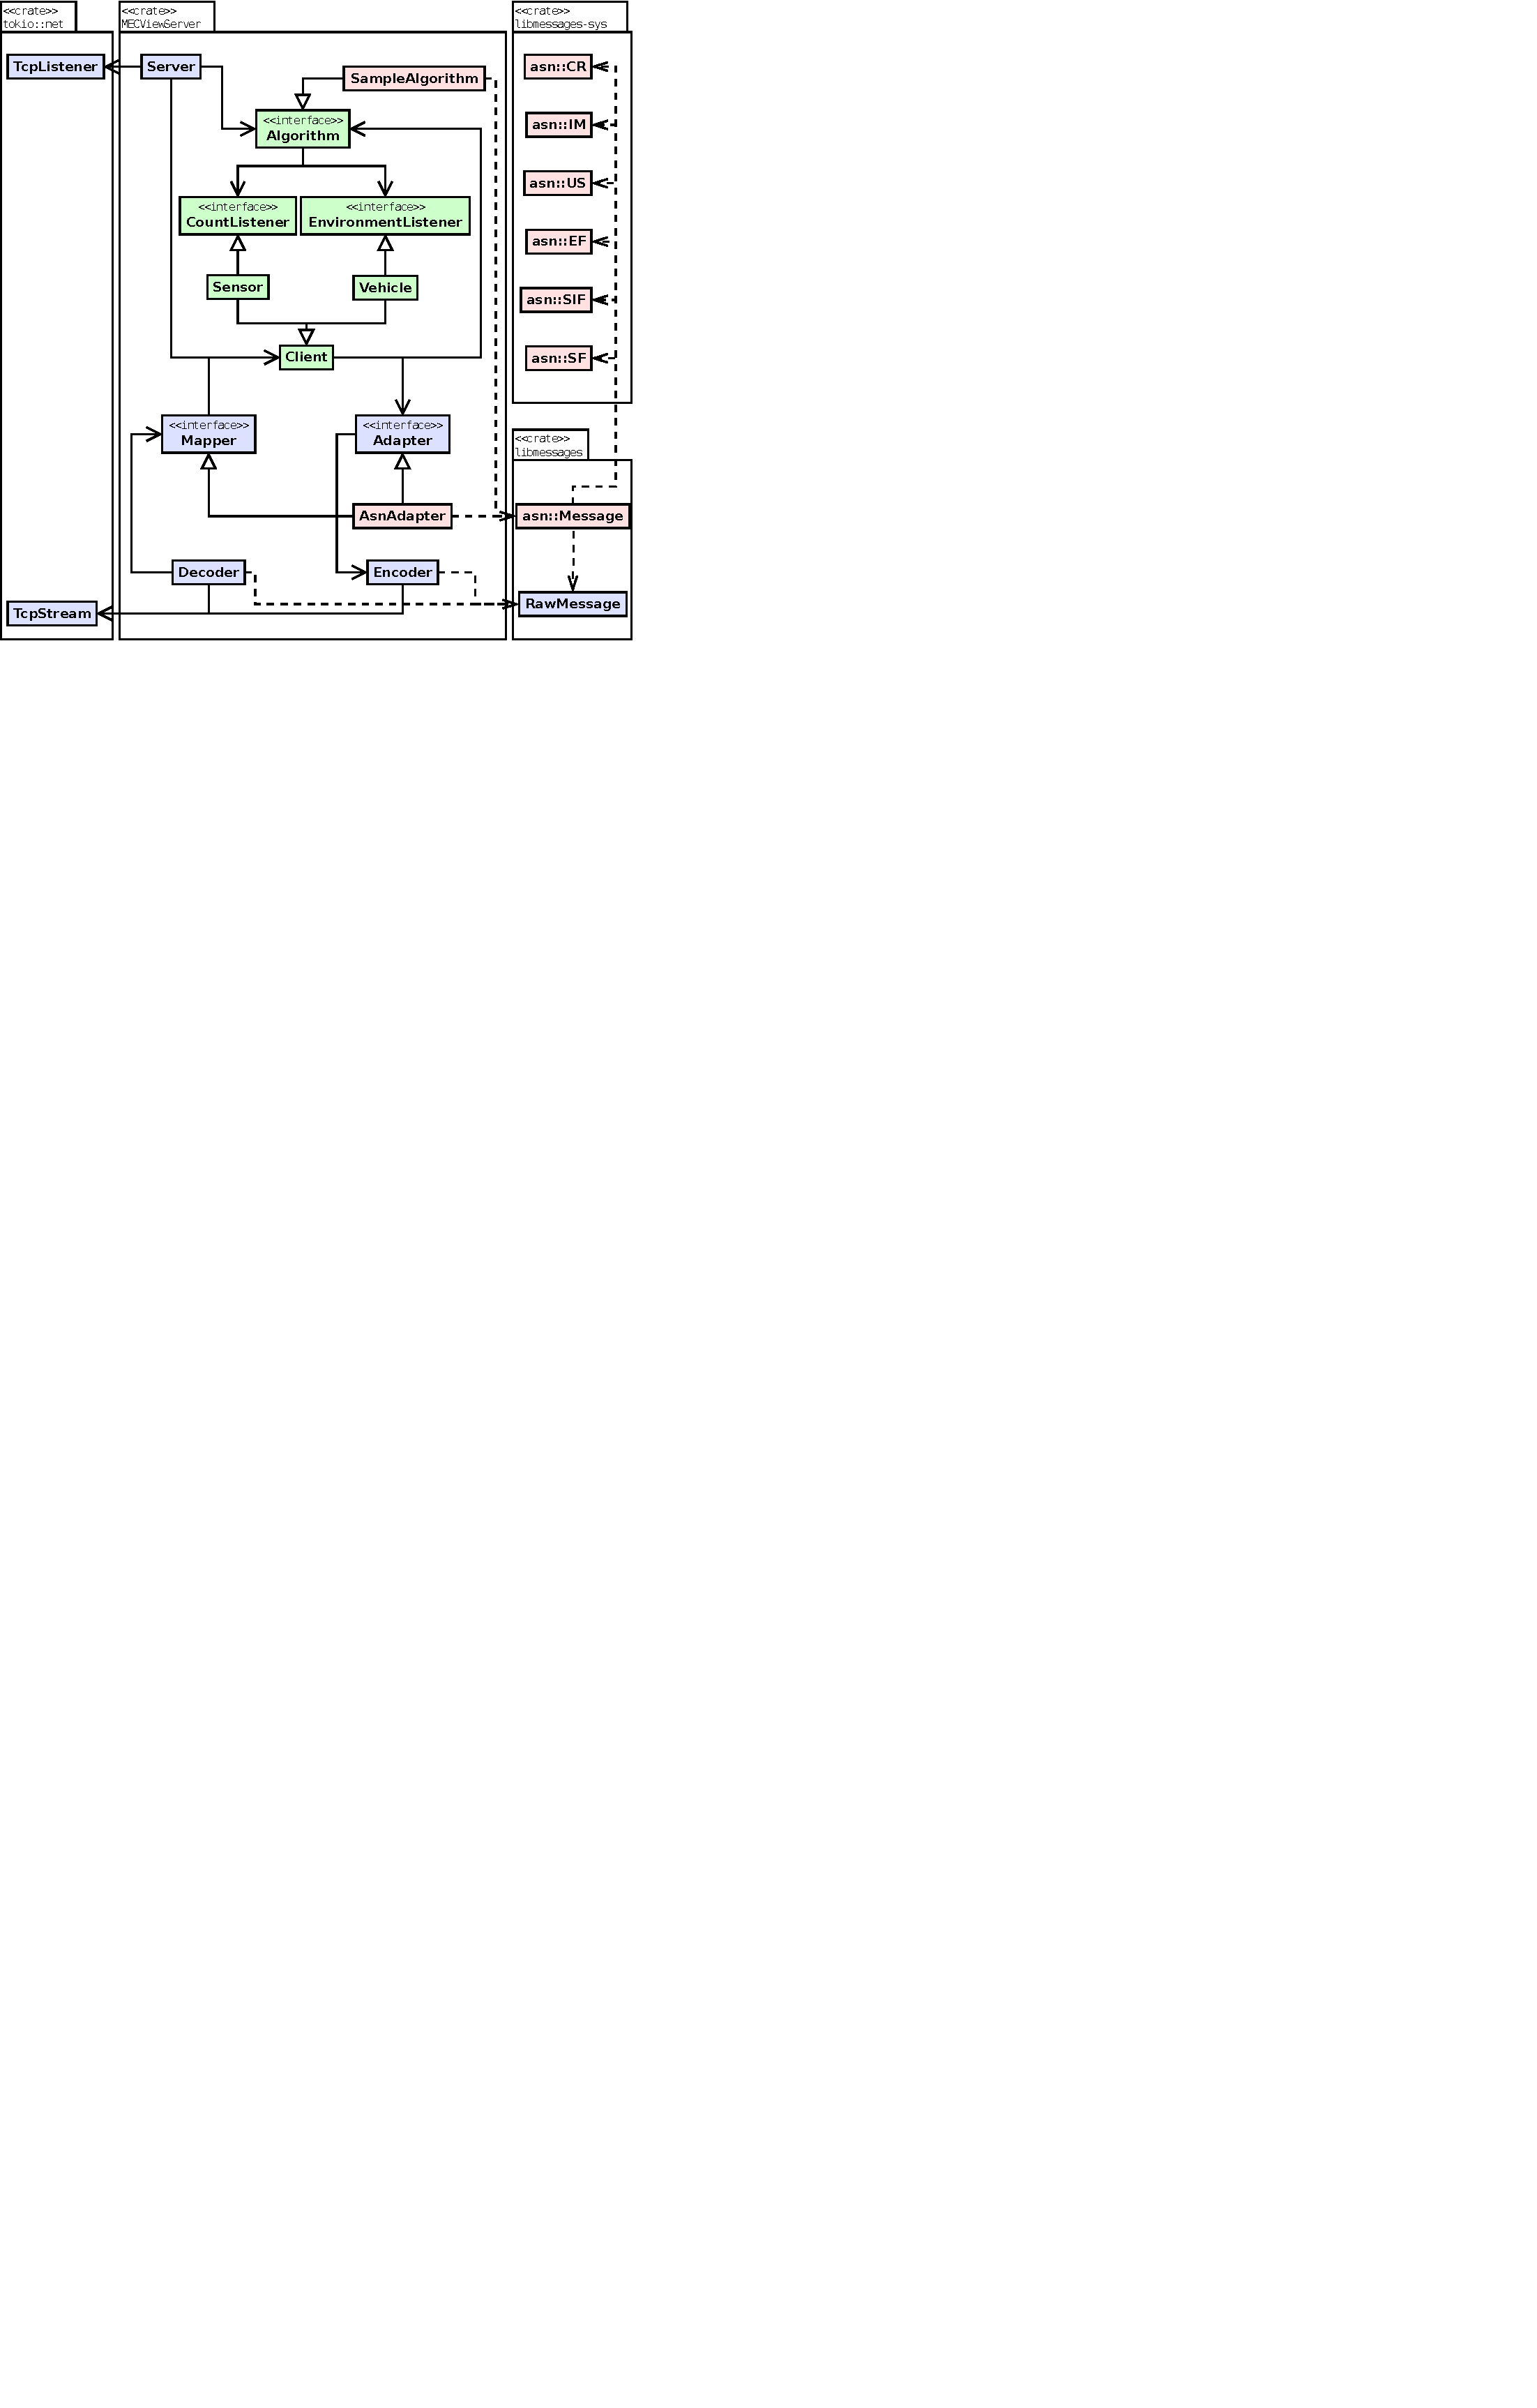
\includegraphics[width=1.9\textwidth]{dia/architecture}
	\caption{Architekturentwurf}
	\label{draft:architecture}
\end{figure}

Die grün und blau markierten Klassen aus \autoref{draft:architecture} haben keine direkten Abhängigkeiten zu den ASN.1 Nachrichtentypen.
Klassen, die eine Nachricht weiterleiten müssen und deshalb einen Berührungspunkt mit diesen haben, verwenden \textit{Generics} (so muss der Client \textit{SensorFrame}-Nachrichten an den Algorithmus weiterleiten, den konkreten Typ jedoch nicht kennen).
Lediglich durch die Nutzung in Kombination mit den ASN.1 Nachrichtentypen entstehen zur Compilezeit Abhängigkeiten, die aufgrund der Übersicht aber nicht eingezeichnet sind.

Die Klasse \textit{RawMessage} aus der Crate \textit{libmessages} ist eine Containerklasse, um binäre Daten mit Typindikatoren zwischen Decoder und Mapper und zwischen Encoder und Adapter auszutauschen.
Die Klasse selbst hat keine weiteren Abhängigkeiten und ist von der eingesetzten Nachrichtentechnologie unabhängig.
Die \textit{asn::Message} soll Methoden bereitstellen, eine Instanz einer ASN.1 Nachricht in eine \textit{RawMessage} zu serialisieren und eine Instanz einer ASN.1 Nachricht aus einer \textit{RawMessage} zu deserialisieren.
% \todo{Kopf / Body \autoref{analysis:messages}}

Die Implementation ist in drei Crates aufgeteilt:
\begin{itemize}
	\item \textbf{libmessages-sys}: Enthält Bindings für die ASN.1 Datenstrukturen und Funktionen der C-Bibliothek (siehe \autoref{rust:ffi}).
	Unsichere Funktionsaufrufe nach C, wie zur Serialisierung und Deserialisierung, sind durch sichere Rust Funktionen gekapselt.
	Eine ordnungsgemäße Allokation und Deallokation der Nachrichten wird hier sichergestellt.
	
	\item \textbf{libmessages}: Stellt Datenstrukturen und Implementationen bereit um unabhängig von der eingesetzten Nachrichtentechnologie eine Nachricht abbilden zu können.
	Hierzu wird in \textit{RawMessage} der Kopf (siehe \autoref{analysis:messages}) und der binären Inhalt einer Nachricht dargestellt.
	
	Zusätzlich ist in dieser Crate für jede verwendete Technologie (in dieser Bachelorarbeit nur ASN.1) die Wandlung zwischen einer \textit{RawMessage} und einer entsprechenden Datenstruktur implementiert.
	
	\item \textbf{MECViewServer}: Enthält die Logik für den Sensor, das Fahrzeug und den Algorithmus und bündelt sie mit der Kommunikationslogik zu einem ausführbaren Kompilat.
	
	\item \textbf{tokio::net}: Diese Crate ist Teil des Frameworks von Tokio (siehe \autoref{design:tokio}) und wird hier lediglich aus Gründen der Vollständigkeit erwähnt.
	Anstatt die TCP-Klassen der Standardbibliothek zu nutzen, werden die erweiterten Versionen von Tokio genutzt.
	Die TCP-Klassen von Tokio können asynchron mittels \textit{Future}s und Kanälen genutzt werden, wie es in der Standardbibliothek (noch \cite{rust:github:futures}) nicht möglich ist.
\end{itemize}

\subsubsection{Erklärung Server}

Der Server instantiiert beim Start einen konkreten Algorithmus, öffnet einen TCP-Port und wartet auf dem daraus resultierenden \textit{TcpListener} auf neue Clients.
Jedem neuen Client wird eine Referenz auf den Algorithmus übergeben und asynchron bearbeitet.

\subsubsection{Erklärung Client, Sensor und Vehicle}

Der Client hält eine Referenz auf einen Algorithmus und einen Adapter.
Im Falle eines \textit{Vehicle}s kann ein \textit{EnvironmentListener} am Algorithmus registriert werden, um neue Umgebungsmodelle zu erhalten.
Im Falle eines \textit{Sensor}s kann ein \textit{CountListener} am Algorithmus registriert werden, um über Änderungen bei der Anzahl der registrierten Fahrzeuge informiert zu werden.

\subsubsection{Erklärung Adapter}

Der Adapter bietet  Schnittstellen, damit eine Client-Instanz Nachrichten versenden kann, ohne die eingesetzte Nachrichtentechnologie zu kennen.
Hierzu wird der Client-Instanz Funktionen bereitgestellt, die von der Adapterimplementation in entsprechende Nachrichten übersetzt werden.

\subsubsection{Erklärung Mapper}

Der Mapper ruft für empfangene Nachrichten der eingesetzten Nachrichtentechnologie Funktionen der Client-Instanz auf und agiert somit als Gegenstück zum Adapter.

\subsubsection{Erklärung Encoder / Decoder}

Der Encoder schreibt \textit{RawMessage}s auf den TCP-Datenstrom, während der Encoder \textit{RawMessage}s vom TCP-Datenstrom liest.
Hierzu wird eine Wandlung, wie in \autoref{analysis:messages} beschrieben, vorgenommen.

\subsubsection{Nachrichtentechnologie kapseln}

Innerhalb der MECViewServer Crate sollen möglichst wenige Klassen die eingesetzt Nachrichtentechnologie kennen.
Hierzu zählen die Algorithmus- (\textit{SampleAlgorithmus}), Mapper- und Adapterimplementationen (\textit{AsnAdapter}).
Dies ist unumgänglich, weil sowohl der eingesetzte Algorithmus, der Mapper und der Adapter Felder einer Nachricht sowohl lesen als auch schreiben muss.
Zudem muss der Server mindestens indirekt die eingesetzte Technologie kennen, um die richtigen und zueinander kompatiblen Algorithmus-, Mapper- und Adapterimplementation zu instantiieren.
Weitere Klassen agieren dagegen unabhängig von der eingesetzten Nachrichtentechnologie.

\subsection{Kommunikationsarchitektur}
\label{design:communication:architecture}
\label{design:communication:architecture:async}

Um ein Mehrkernsystem effizient zu nutzen, arbeiten einige Klassen asynchron zueinander.
Hierzu zählt der Server, der fortlaufend neue Verbindungen annimmt.
Die daraus resultierenden Client-Instanzen bearbeiteten asynchron eingehende Anfragen.
Letztendlich aktualisiert auch der Algorithmus asynchron zu den Client-Instanzen und dem Server das Umfeldmodell.

Die Kommunikation zwischen einem TCP-Datenstrom und einer Client-Instanz soll mittels des \enquote{Channel Architektur Pattern} \cite[157]{douglass2003real} verwirklicht werden.
Das Muster eignet sich besonders gut, da auf eingehende und ausgehende Datensätze eine immer gleiche Transformation angewandt werden muss:

\begin{figure}[h]
	\centering
	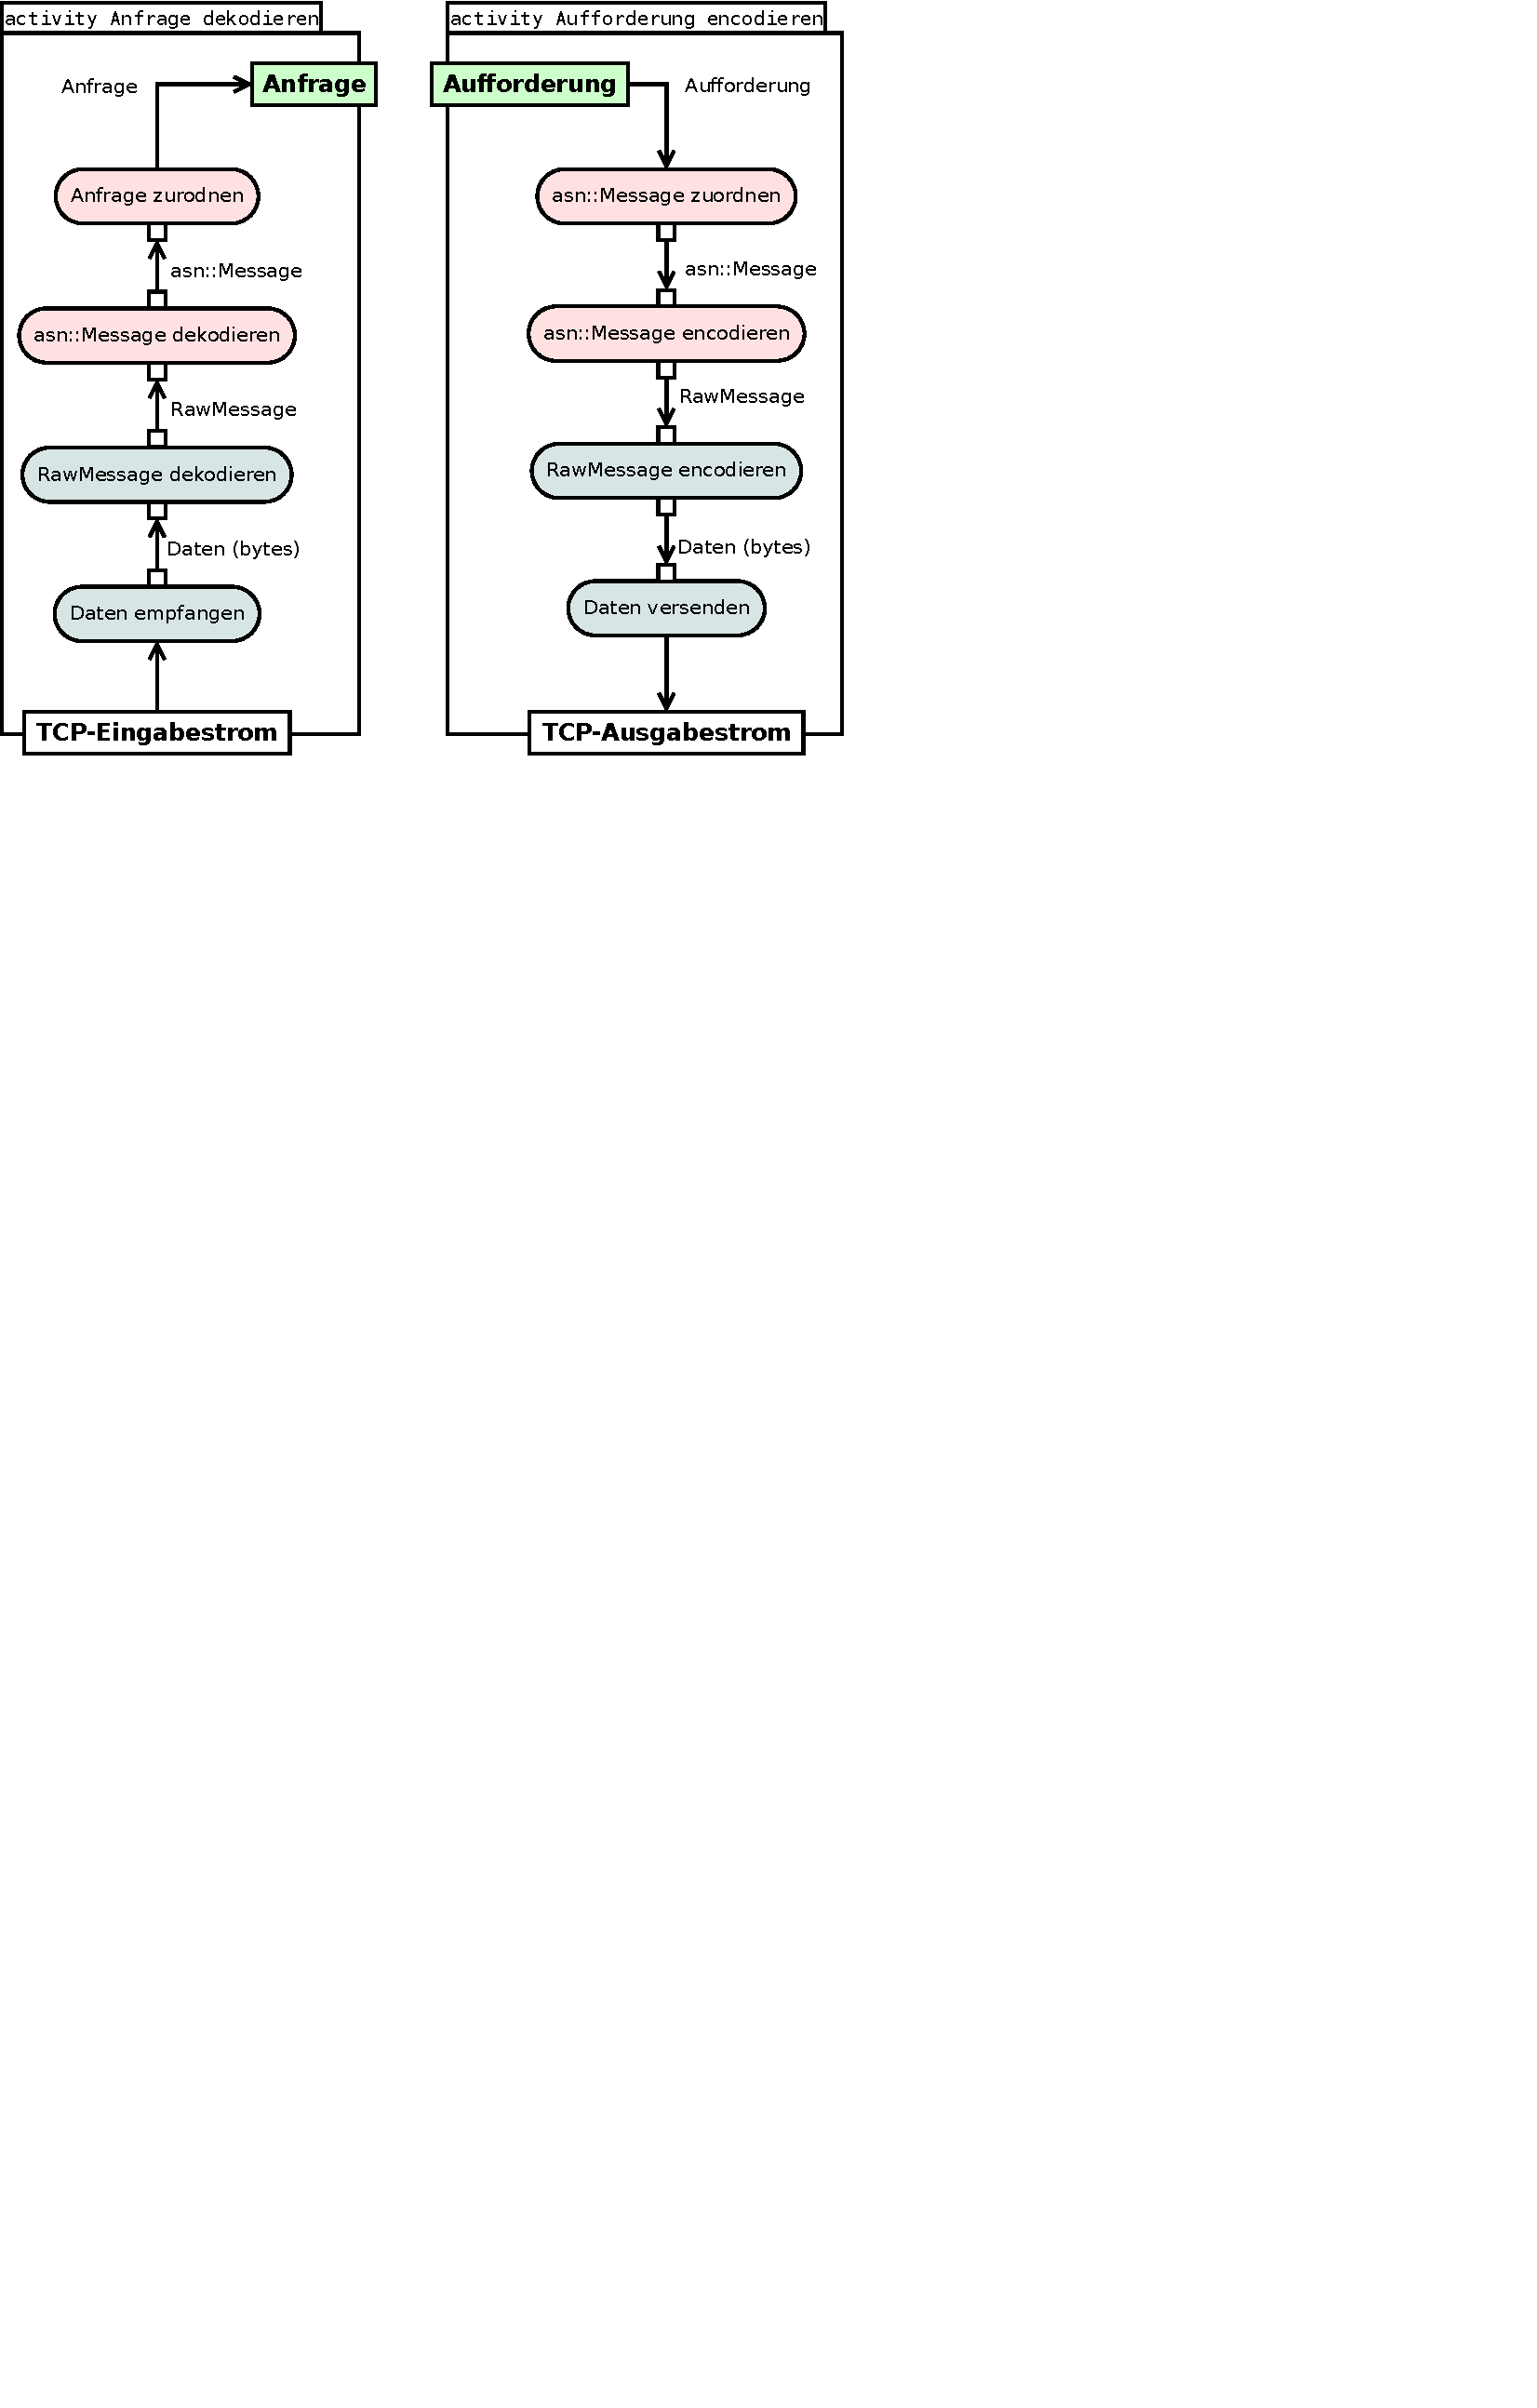
\includegraphics[width=1.4\textwidth]{dia/channel_sep}
	\caption{Aktivitätsdiagramme zum Dekodieren einer Anfrage aus dem TCP-Datenstrom (unten) und zum Versenden einer Aufforderung (oben).}
	\label{design:channel}
\end{figure}

Die Aktivitätsdiagramme in \autoref{design:channel} beschreiben die nötigen Transformationen, um eine empfangene Anfrage zu dekodieren und um eine Aufforderung zu encodieren und zu versenden:

\begin{itemize}
	\item \textbf{Daten empfangen}: Die eingehenden Daten (hier Bytes) müssen angesammelt werden, bis sie eine komplette Anfrage abbilden.
	\item \textbf{RawMessage dekodieren}: Die angesammelten Daten werden in eine RawMessage gewandelt. Nachrichtentyp und Inhalt werden hierbei extrahiert.
	\item \textbf{asn::Message dekodieren}: Aus dem Inhalt wird eine ASN-Nachricht des entsprechenden Typs dekodiert.
	\item \textbf{Anfrage zuordnen}: Die ASN-Nachricht wird einer Anfrage zugeordnet.
	\item \textbf{asn::Message zuordnen}: Die Aufforderung wird in eine ASN-Nachricht eingebettet.
	\item \textbf{asn::Message encodieren}: Die ASN-Nachricht wird in eine RawMessage encodiert. Der Nachrichtentyp wird entsprechend gesetzt.
	\item \textbf{RawMessage encodieren}: Die RawMessage wird in Bytes gewandelt.
	\item \textbf{Daten versenden}: Die Bytes werden über den TCP-Datenstrom versandt.
\end{itemize}

Nach dem \enquote{Channel Architektur Pattern} ist eine sequentielle Bearbeitung zwischen dem TCP-Datenstrom und der Client-Instanz in jede Richtung als Kanal interpretierbar (sprich jedes Aktivitätsdiagramm aus \autoref{design:channel}).
Da jeder Zwischenschritt innerhalb eines Kanals lediglich vom Ergebnis des vorhergehenden abhängig ist, könnten die einzelnen Schritte parallel zueinander bearbeiten werden.
Durch einen zusätzlich vorangestellten Multiplexer und nachfolgenden Demultiplexer könnten zudem mehrere Kanäle parallel die Client-Instanz oder den Datenstrom speisen.
Hiervon wird in der ersten Implementierung jedoch abgesehen, da je Client keine derart große Datenflut erwartet wird.
Stattdessen werden viele Clients erwartet, weshalb jeder Kanal eines Clients parallel zu den Kanälen anderer Clients ausgeführt werden soll.

Als Framework zur Umsetzung wird \textit{Tokio} (siehe \autoref{design:tokio}) verwendet.
Durch die Kombinationsmöglichkeiten von \textit{Future}s und nicht blockierenden Kommunikationskanälen ermöglicht es, ein System nach diesem Prinzip zu erstellen.

%Bei einer großen Datenmenge kann dies helfen, die Anforderungen von echtzeitnahen System zu erfüllen (\cite[161]{douglass2003real}).

%Das \enquote{Channel Architektur Pattern} \cite[157]{douglass2003real}, welches bereits von \textit{Tokio} (siehe \autoref{design:tokio}) verwendet wird, wird dies ermöglichen.

%\todo{explain more channel system}



%\todo{Abbildung vereinfacht, Kommunikation via Queues im tokio context}
%~\\ ~\\ ~\\




%?? 
%\todo{Komponentendiagramme bei \cite[446]{goll2012methoden}, example \cite[457]{goll2012methoden}, tikz-uml: server, algorithm, encoder/...}		



%\section{..}

%\todo{Design Pattern, Gamma et al, four important aspects}

%\todo{Real Time Design Patterns Buch: Ab Seite 141, verschiedene Systempatterns, microkernel \cite[151]{douglass2003real}? channel architektur pattern \cite[167]{douglass2003real}?}
